% !Mode:: "TeX:UTF-8"
\documentclass{../../common/tufte-latex/tufte-handout}

\title{Git hands-on, part I: Introduction \& Installation}
\author{S\'ebastien Dawans}

%\date{21 January 2014} % without \date command, current date is supplied

%\geometry{showframe} % display margins for debugging page layout
\usepackage[utf8]{inputenc}
\usepackage{graphicx} % allow embedded images
  \setkeys{Gin}{width=\linewidth,totalheight=\textheight,keepaspectratio}
  \graphicspath{{graphics/}} % set of paths to search for images
\usepackage{amsmath}  % extended mathematics
\usepackage{booktabs} % book-quality tables
\usepackage{units}    % non-stacked fractions and better unit spacing
\usepackage{multicol} % multiple column layout facilities
\usepackage{lipsum}   % filler text
\usepackage{fancyvrb} % extended verbatim environments
  \fvset{fontsize=\normalsize}% default font size for fancy-verbatim environments
\usepackage{listings}
\lstset{showstringspaces=false}
\usepackage[usenames]{xcolor}
\usepackage{hyperref}

\lstdefinestyle{BashInputStyle}{
  language=bash,
  basicstyle=\footnotesize\ttfamily,
  %numbers=left,
  %numberstyle=\tiny,
  %numbersep=3pt,
  frame=tb,
  columns=fullflexible,
  backgroundcolor=\color{yellow!20},
  linewidth=0.95\linewidth,
  xleftmargin=0.05\linewidth,
  moredelim=**[is][\color{red}]{§}{§},
  moredelim=**[is][\color{OliveGreen}]{`}{`}
}

% Standardize command font styles and environments
\newcommand{\doccmd}[1]{\texttt{\textbackslash#1}}% command name -- adds backslash automatically
\newcommand{\docopt}[1]{\ensuremath{\langle}\textrm{\textit{#1}}\ensuremath{\rangle}}% optional command argument
\newcommand{\docarg}[1]{\textrm{\textit{#1}}}% (required) command argument
\newcommand{\docenv}[1]{\textsf{#1}}% environment name
\newcommand{\docpkg}[1]{\texttt{#1}}% package name
\newcommand{\doccls}[1]{\texttt{#1}}% document class name
\newcommand{\docclsopt}[1]{\texttt{#1}}% document class option name
\newenvironment{docspec}{\begin{quote}\noindent}{\end{quote}}% command specification environment



\begin{document}

\maketitle% this prints the handout title, author, and date

\begin{abstract}
\noindent
This handout introduces the Git Source Code Management Tool and provides installation instructions which should ideally be done by anyone following sessions from UseGit.com \marginnote{\color{blue}\underline{\url{http://www.usegit.com}}} prior to the first lesson.

The goal is to offer a first experience with Git on the client side using Git's native command-line interface to learn basic concepts about Source Code Management with Git.
The intended audience for this session is one or more developers having already received in introduction to basic Git concepts, such as those available in the presentations folder of the git-slides repository \marginnote{All course handouts and presentations are freely available at {\color{blue}\underline{\url{https://github.com/sdawans/git-slides}}}}.

\end{abstract}

%\printclassoptions

\section{Introduction}\label{sec:intro}

Git is a Source Code Management (SCM) system with three key design principles.
Git is \textbf{Distributed}, \textbf{Fast} and \textbf{Reliable}.
It is very different from not only centralized SCMs like SVN, but also other forms of distributed SCMs like Mercurial.
To follow this introductory session, it's best to clear your mind of everything you know about other SCMs, as some false similarities are often misleading.

\section{Installation: command-line Git}

In preparation of this course, each participant should have a properly installed and configured command-line client for Git, and access to the git repositories hosted on a local instance of git hosting solution such as Gitlab or Gitolite.

Although there exist some graphical clients for git such as SourceTree, SmartGit, Tower, etc, I prefer to give lessons using the Git command line. There are several reasons for this:

\begin{enumerate} 
 \item{\textbf{GUIs hide the basic Git commands}. Getting comfortable with Git requires some insight on how the tool works. This also means learning the basic vocabulary which mostly corresponds to knowing some of the basic git commands, often abstracted in GUIs.}
 \item{\textbf{GUIs automate things}. \marginnote{This is especially true when working with submodules - it is practically impossible to learn how submodules work without the command-line} GUIs sometimes combine several Git commands into one.  That may be fine for some use-cases, but it also means sacrificing some flexibilty and problem-solving techniques.}
 \item{\textbf{GUIs won't help when you're stuck}. \marginnote{When someone asks for help, I usually start by opening a Git shell.} Every once in a while, even the most seasoned Git user will run into some unexpected situations. From my experience, it is a lot simpler to analyse and problem-solve in a command-line then in a GUI.}
 \item{\textbf{Easier to learn in a group}. It's also just simpler to follow a group lesson when everyone uses the same client. Command-line clients ensure a common experience for all attendees.}
\end{enumerate}

That said, graphical tools can still bring a lot of value to your Git workflow later on once you are acquainted with the basic commands.

\subsection{Installing a Git client on MacOS X and Linux}

Linux and MacOS X users will find the native git client in their respective package managers.

Git clients on some linux distributions may be slightly outdated compared to the latest Windows binaries, \marginnote{\url{https://git-scm.com/book/en/v2/Getting-Started-Installing-Git}} so it can be a good idea to install git from source. However, this is not strictly necessary for following the following courses.

\subsection{Installing a Git client on Windows}\label{sec:preparation}

Windows users should install the latest versions of TortoiseGit \marginnote{\url{http://code.google.com/p/tortoisegit/}} (for the TortoisePlink.exe binary) and msysgit \marginnote{\url{http://code.google.com/p/msysgit/}}, in that order.
Furthermore, windows users will need puttygen.exe and pageant.exe, available on the Putty website \marginnote{\url{http://www.putty.org/}}. These should be stored somewhere on disk, I usually put them in:

\begin{lstlisting}[style=BashInputStyle]
  C:\bin\ssh\
\end{lstlisting}

\begin{itemize}

\item{An SSH keypair must be generated with puttygen.}
\item{The public key displayed in the puttygen GUI should be copy/pasted in your Git Repository Server user settings (GitHub, Gitlab, Gitolite, Redmine...) while the private key should be stored locally and added to pageant.} \marginnote{When pasting the public key in Gitlab, make sure you copy it directly from the puttygen application, and not from the public key file saved on disk. This avoids problems caused by tools requiring the OpenSSH format.}
\item{Optionally, you may want to write a batch script to automatically run pageant at system boot and load the private key.}
\item{Create a new environment variable called GIT\_SSH, poiting to the TortoisePlink.exe binary, which should be located in:}

\begin{lstlisting}[style=BashInputStyle]
  GIT_SSH = C:\Program Files\TortoiseGit\bin\TortoisePlink.exe
\end{lstlisting}

\item{After creating this environment variable, you must close and re-open your Git shells for the variable to get loaded. In Git Bash, you can verify the value of GIT\_SSH:}

\begin{lstlisting}[style=BashInputStyle]
  $ echo $GIT_SSH
  C:\Program Files\TortoiseGit\bin\TortoisePlink.exe
\end{lstlisting}

\end{itemize}

\subsection{Configuring Git}

People are an important aspect in any SCM, as every code change must be attributed to a certain author.
\marginnote{In fact, Git manages users thoroughly by seperating \textbf{authors} from \textbf{committers}.
An author is the person who (originally) writes a certain patch (new code, code modification), while the committer is the person who applies the said changes on a particular code base.}
The user must thus identify himself before using a git client.
Git uses a global \texttt{user.name} and \texttt{user.email} setting applied to all projects, which is overridable locally for a specific project.
For this session, we will set the global settings for all the projects on the machine:

\begin{lstlisting}[style=BashInputStyle]
  $ git config --global user.name "First Last"
  $ git config --global user.email "first.last@example.com"
\end{lstlisting}

Another useful configuration (already default on msysgit) is to enable color output in the console.

\noindent To do so:

\begin{lstlisting}[style=BashInputStyle]
  $ git config --global color.ui true
\end{lstlisting}

Windows users who are not comfortable with Vim, the default commit-message editor in msysgit, can define a \texttt{core.editor} option to another editor.
For example, to use Notepad++ as default:

\marginnote{According to \url{http://starikovs.com/2012/11/06/git-core-editor-windows/}, you can simple write 'notepad++' instead of the full path to the application if it is correctly defined in your PATH environment variable.}
\begin{lstlisting}[style=BashInputStyle]
  $ git config --global core.editor
    "'C:/path/to/notepad++.exe' -multiInst -notabbar -nosession -noPlugin"
\end{lstlisting}

At this point, it is worth noting that the above \texttt{git config} commands using the \texttt{--global} option store client-wide configurations in a file located in:

\begin{lstlisting}[style=BashInputStyle]
  ~/.gitconfig
  --> C:\Users\MyLogin\.gitconfig  # on Windows
  --> /home/user/.gitconfig        # on Linux
\end{lstlisting}

Without the \texttt{--global} option, the \texttt{git config} command applies settings at the repository level, and override and existing global configuration in case of duplicates. The repository config file is in:

\begin{lstlisting}[style=BashInputStyle]
  root_folder/.git/config
\end{lstlisting}

\noindent Either of these files can be opened directly for editing using: \marginnote{A google search for \textbf{git dotfile} will show you a lot of examples of aliases which can be useful to define in the global configuraiton file. However, like for the GUIs, it's best to start with the raw git commands while learning.}

\begin{lstlisting}[style=BashInputStyle]
  git config [--global] --edit
\end{lstlisting}

\noindent For a full list of global and locally overridden parameters, use

\begin{lstlisting}[style=BashInputStyle]
  $ git config --list
\end{lstlisting}

Finally, a useful configuration before getting started is \textbf{shell prompt customization}.
Windows users using msysgit already have a very basic form of preconfigured customization. \marginnote{Git Prompt: \url{http://volnitsky.com/project/git-prompt/}}
For Unix-based systems, I recommend the highly configurable git-prompt project. 

%TODO: make my notes on git-prompt public and add a link to it

\subsection{Recommended Repository Hosting Solutions}

As most of these courses are given to companies, it is often necessary to discuss the possible solutions for hosting Git repositories.

\textbf{Gitlab}

\marginnote{My feedback on GitLab [FR] \url{https://www.cetic.be/Solution-Open-Source-et-complete-d}}
\begin{marginfigure}%
  \centering
  
\includegraphics[width=0.6\linewidth]{gitlab-logo.png}
  \label{fig:gitlablogo}
\end{marginfigure}

\noindent Gitlab is a popular free open-source Git hosting solution, providing an experience similar to Github but with the advantage of being hosted internally in a company and fully private.

Gitlab offers a web interface to manage and visualize the git repositories hosted on the Git server.
Each git repository hosted on Gitlab can be visualized via a unique URL, usually \\ \noindent \texttt{http://gitlab.server.com/namespace/project}.
The \textbf{namespace} can be of two types: user-owned namespaces, which are the user logins, or group namespaces.
Although \marginnote{\color{blue}\underline{\url{https://bitnami.com/stack/gitlab}}} the official Gitlab installation and migration scripts are quite easy to use, some users might prefer to download a ready-made Gitlab image such as those provided by bitnami.

\textbf{Redmine + Gitolite}

\begin{marginfigure}%
  \centering
  
\includegraphics[width=0.6\linewidth]{redmine-logo.png}
  \label{fig:gitlablogo}
\end{marginfigure}

\noindent Redmine is a popular project management tool, which supports Gitolite integration using the Redmine Git Hosting plugin. \marginnote{Redmine Git Hosting \url{https://www.redmine.org/plugins/redmine_git_hosting}}. This installation is trickier than Gitlab and should only be attempted by an experiences System Administrator.

\subsection{Testing the SSH connection to the Git repositories}

The last configuration step consists in checking  that the network connexion to the Git server is functional.
\begin{marginfigure}%
  \centering
  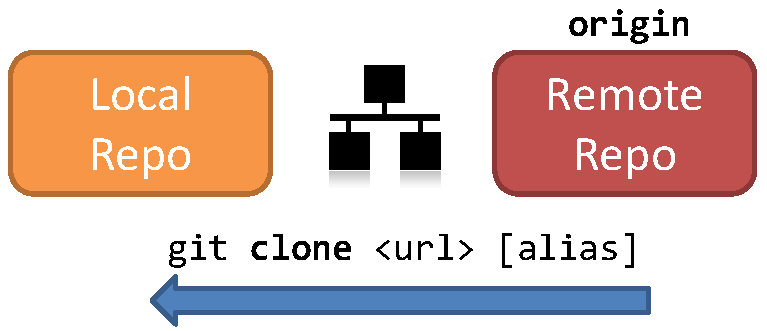
\includegraphics[width=\linewidth]{gitclone-schema.pdf}
  \label{fig:gitclone}
\end{marginfigure}
\marginnote{An optional folder name can be supplied as last argument to rename the top-level directory of the git repository.}
\marginnote{The SSH protocol is implied when using the user@server URL formatting. It is equivalent to ssh://user@server}
We can try to \textbf{clone} an existing Git repository for that.
In the Git jargon, \texttt{clone} consists in copying the entire Git repository from the remote server to the local machine.
As opposed to some centralized SCM tools like SVN, \texttt{git clone} by default will copy every single piece of information necessary to restore all previous versions ever known.
This is why we say Git is distributed: repositories are completely replicated on every machine.

\begin{lstlisting}[style=BashInputStyle]
  $ git clone git@gitlab.server.com:login/lesson1 [folder]
\end{lstlisting}

\noindent When the connection is successful, git will clone the repository and give a quite verbose output on what is going on:

\begin{lstlisting}[style=BashInputStyle]
  Cloning into 'lesson1'...
  remote: Counting objects: 23, done.
  remote: Compressing objects: 100% (17/17), done.
  remote: Total 23 (delta 3), reused 0 (delta 0)
  Receiving objects: 100% (23/23), done.
  Resolving deltas: 100% (3/3), done.
\end{lstlisting}

A new folder \texttt{lesson1} should appear in the current directory.
The Git repository (\texttt{.git folder}) and working tree are both contained inside the \texttt{lesson1} directory.
\marginnote{\texttt{lesson1}, like all Git repositories, is self-contained and can be moved around the filesystem without risk.}

\marginnote{The \texttt{.git} folder is the actual repository with all Git objects and settings. We will not go into more details about this in this course, and will ignore it hereafter}
\begin{lstlisting}[style=BashInputStyle]
  $ cd lesson1/
  $ tree -L 2 -a 
  .
  |-- .git
  |   |-- branches
  |   |-- config
  |   |-- description
  |   |-- HEAD
  |   |-- hooks
  |   |-- index
  |   |-- info
  |   |-- logs
  |   |-- objects
  |   |-- packed-refs
  |   `-- refs
  |-- python
  |   `-- calc.py
  `-- README.md
\end{lstlisting}

The \textbf{working tree} is the set of files and folders contained inside the \texttt{lesson1} folder, not including the \texttt{.git}.
\begin{marginfigure}%
  \centering
  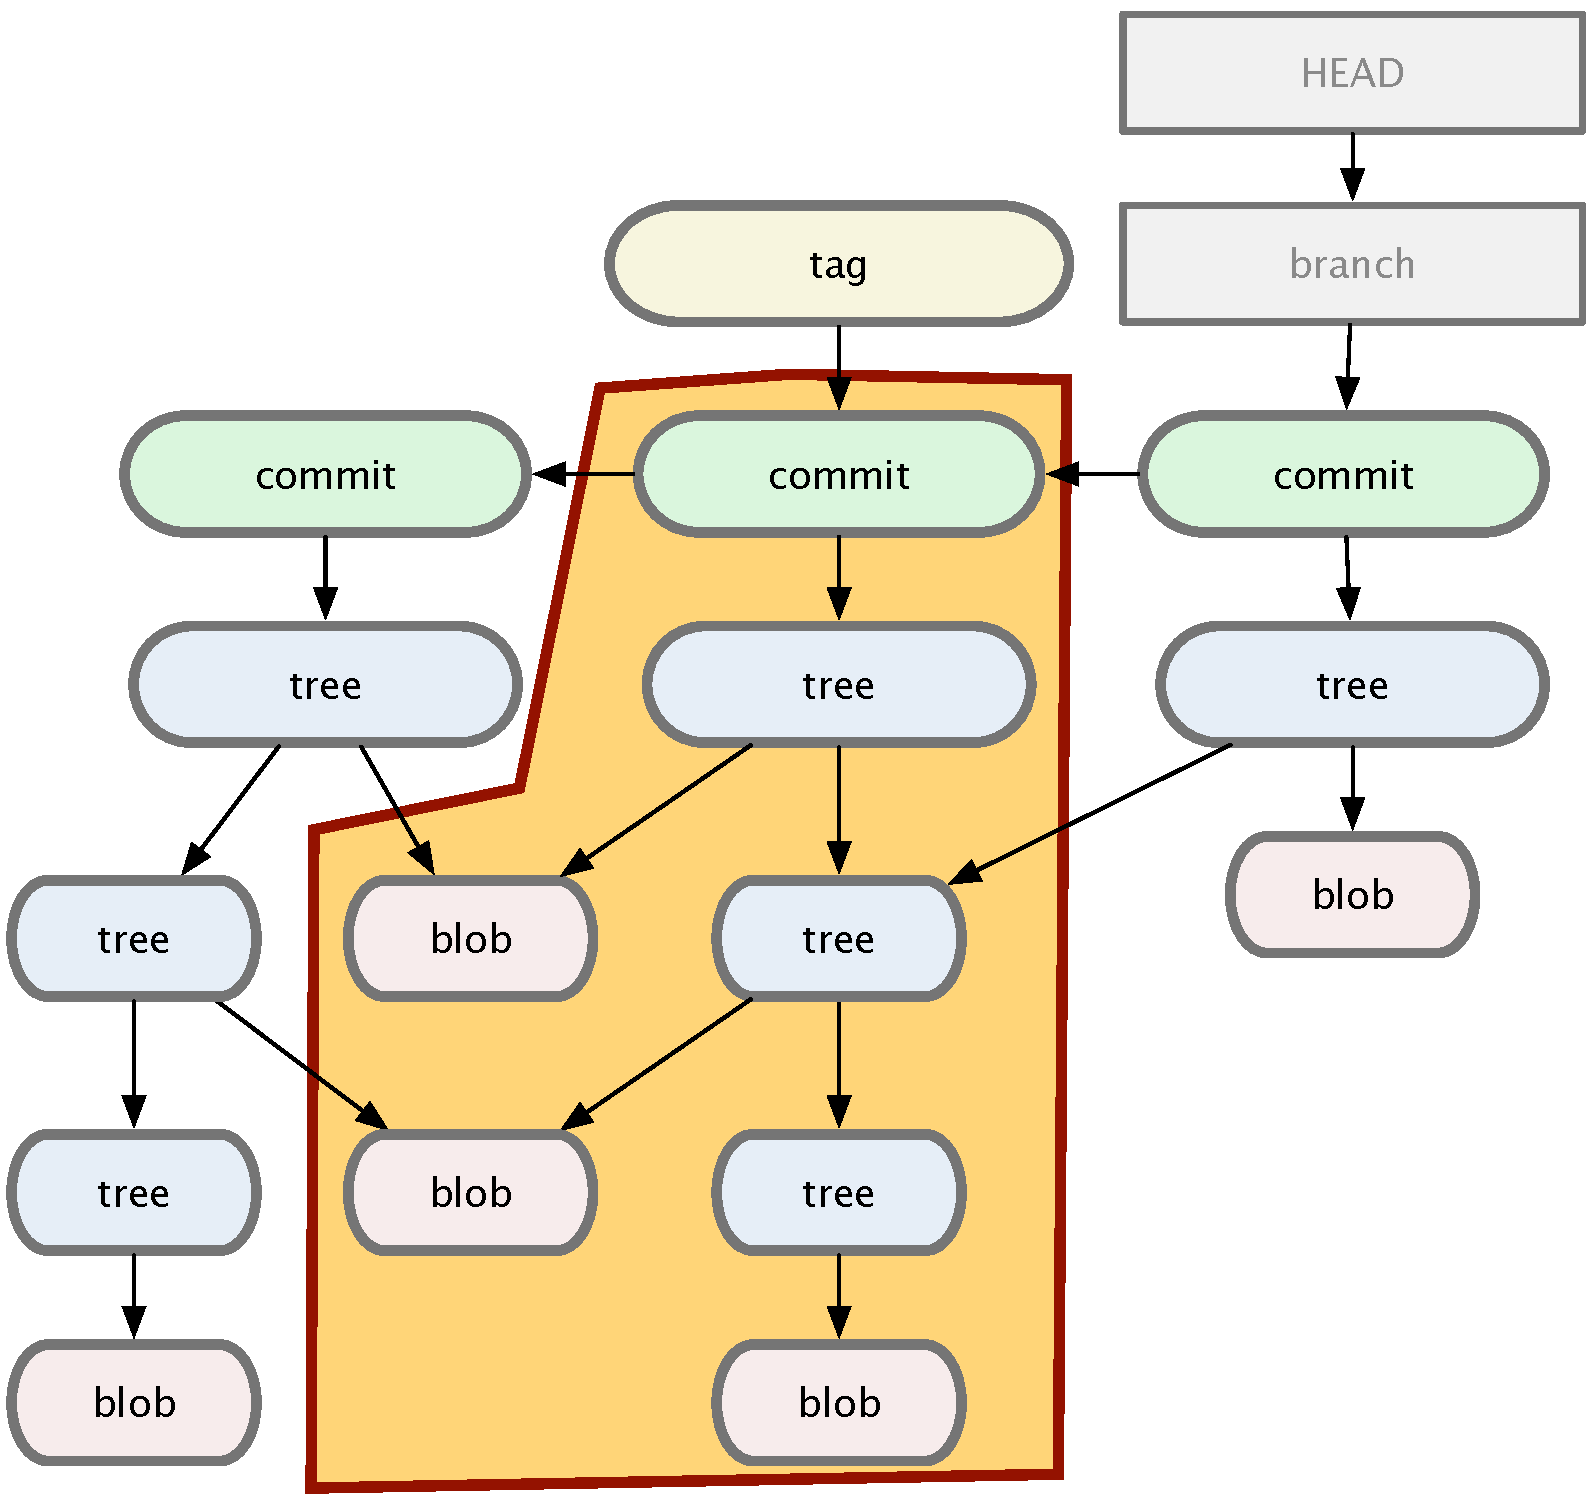
\includegraphics[width=\linewidth]{tree.pdf}
  \label{fig:tree}
  \caption{Representation of an arbitrary working tree for a certain commit. The files checkout out on disk and their folders are represented by blob and tree objects.}
\end{marginfigure}
In our working tree, we have a file called \texttt{README.md} in the root directory, and a \texttt{python} directory containing a single python script.
Only a single \textit{version} of the working tree can be \textit{checked out}, or "on disk" at a given time.

As we have seen in the introductory slides, the working tree is a snapshot of the whole project at a certain point of the history.
A version is uniquely identified by a \textbf{commit} object, containing author/date information and pointing to a top-level \textbf{tree} object and one or more \textbf{parent commits}.
In turn, each \textbf{tree} object contains other \textbf{tree} objects and \textbf{blob} objects, or files.
This course does not cover internal of Git, but you can find more information on Git Objects in the introductory presentation.

\section{Further Reading}

The next session, \texttt{Part II: Single User Operations}, introduces most of the basic git commands. It is designed to become familiar with Git through practice and without (yet) the complexity of managing multiple users in a workflow. Workflows are described in detail in Part III.

\bibliography{tufte-latex/sample-handout}
\bibliographystyle{plainnat}



\end{document}
